\Chapter{Tesztek}
\label{Chap:tesztek}

%A játékmotor vizsgálata egy az egyben
%Review jellegű észrevételek
%Profilozás

Ez a fejezet az általam írt játékmotor, illetve az azzal megvalósított funkciók különböző megvalósításainak tesztjeiről szól. Különböző elemeket, különféle módszerrel lehet implementálni, többféleképp lehet optimalizálni, amelyek kirajzolási idejében különbségek vannak. Léteznek kisebb és nagyobb hatékonyságú algoritmusok a különböző problémák megoldására.

\section{Kirajzolási módszerek}

Alapvetően két fő kirajzolási módszer létezik az OpenGL-ben. Az egyik a régebbi glBegin-glEnd blokkos, a másik a modernebb Vertex Buffer Object-es (VBO). A kettő között a legfőbb különbség a gyorsaság. VBO-s megjelenítési mód esetén, mint ahogy a nevében is benne van, egy buffer-be (tárólóba) betöltjük az összes kirajzolni kívánt elemet, és azt egyben adjuk át a videokártyának, a legmegfelelőbb formátumban. Ez sokkal gyorsabb, mivel a régebbi egyesével adja át a pontokat kirajzolásra. \Aref{fig:old_fps}-es ábrán a régebbi, \aref{fig:vbo_fps}-es  ábrán pedig a VBO-s megjelenítési mód látható. Ugyanazoknak az objektumoknak a kirajzolása sokkal gyorsabb VBO-val, ez látható mindkét képen a bal felső sarokban. Sokkal jobb a hardver kihasználtsága is, és az FPS (képkocka/másodperc) is kicsivel több, mint 8x magasabb.

\begin{figure}[h]
\centering
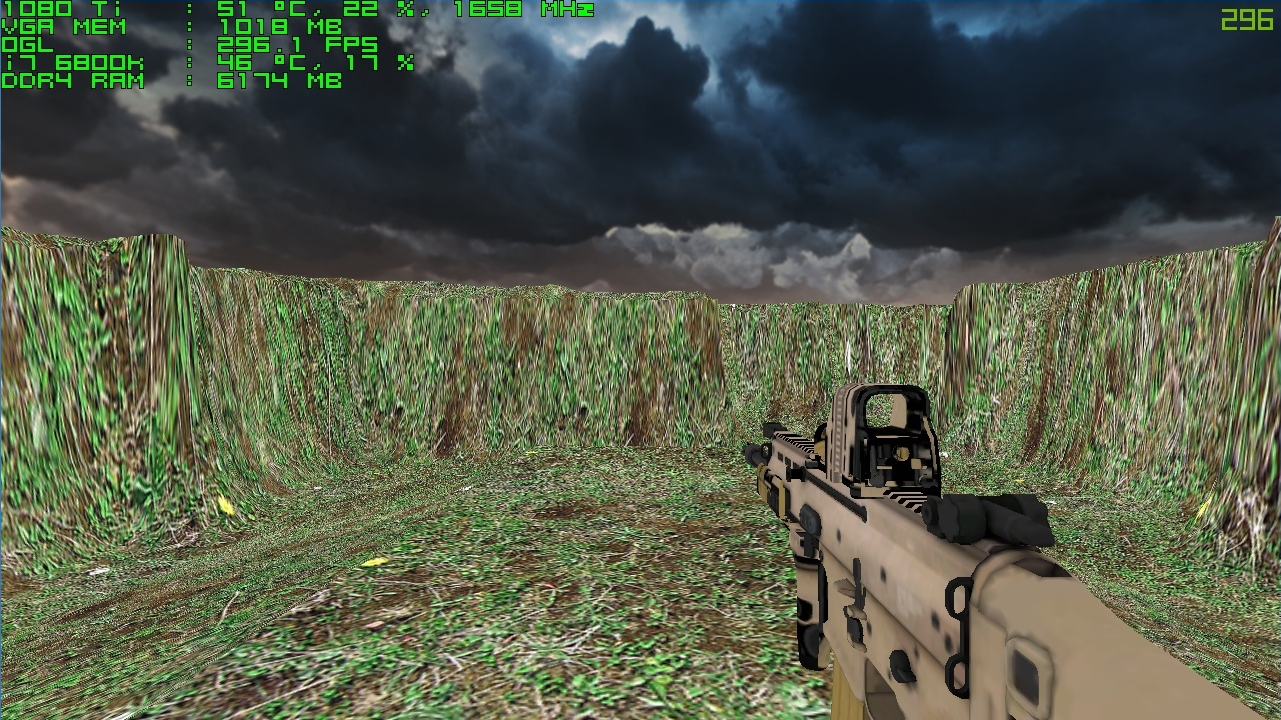
\includegraphics[scale=0.34]{kepek/old_method_fps.png}
\caption{A terep kirajzoltatása a régebbi módszerrel}
\label{fig:old_fps}
\end{figure}

\begin{figure}[h]
\centering
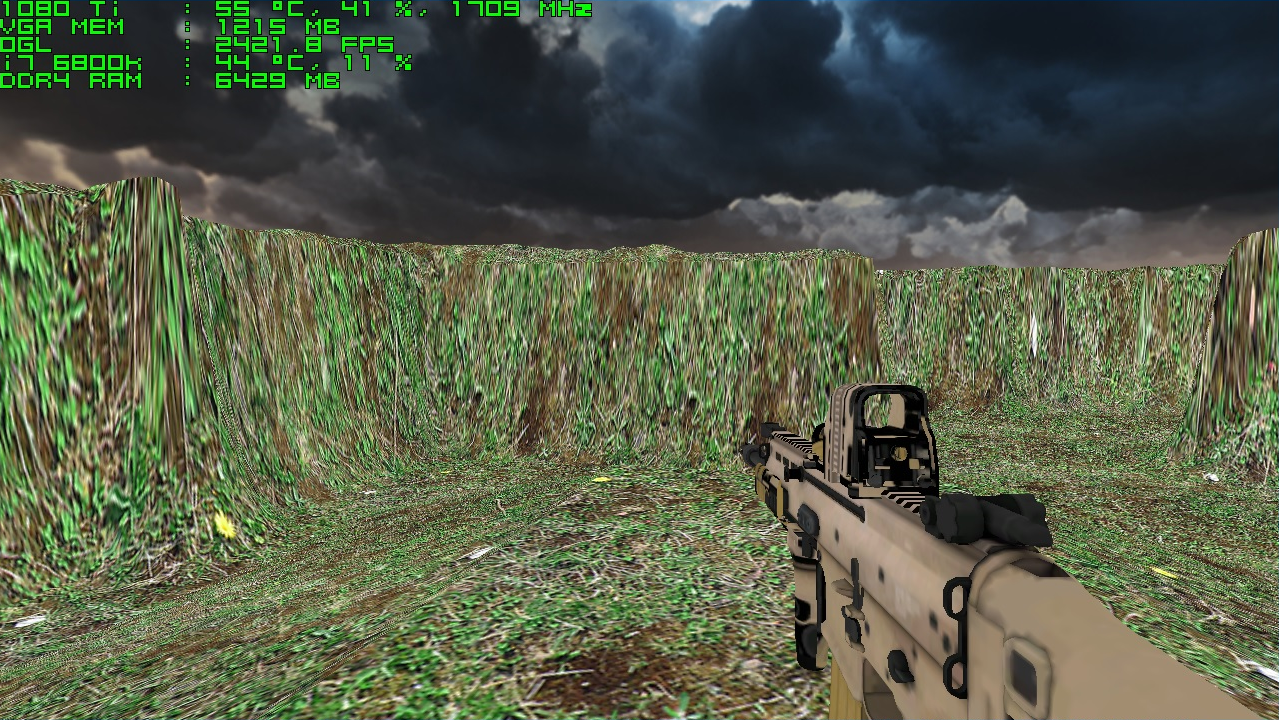
\includegraphics[scale=0.34]{kepek/vbo_method_fps.png}
\caption{A terep kirajzoltatása az újabb, VBO-s módszerrel}
\label{fig:vbo_fps}
\end{figure}

\section{Profilozás}

A játék egyes elemeinek betöltéséről, kirajzolásáról diagramok készültek. Minden ábrán, a függőleges tengelyen az adott objektum, vagy elem neve látható, a vízszintes tengelyen pedig az idő van feltüntetve milliszekundumban.

\Aref{fig:start_diag}-as ábra a játékindítás folyamatának időigényét részletezi, hogy az egyes elemek létrehozása, betöltése hogyan oszlik el a teljes időhöz képest. Mint látható, az időtartam nagy részét a képi elemek betöltése teszi ki, a további négy elem szinte elhanyagolható ilyen szempontból.

\begin{figure}[h]
\centering
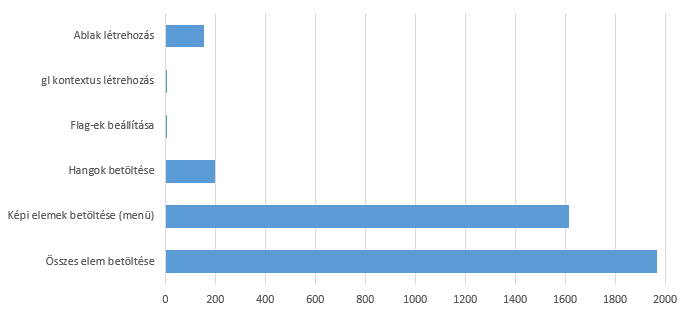
\includegraphics[scale=0.84]{kepek/start_diag.png}
\caption{Játékindítás teljes ideje a menübe való eljutásig}
\label{fig:start_diag}
\end{figure}

\Aref{fig:map_diag}-es ábrán a teljes játéktér betöltésének, illetve az egyes részek betöltésének ideje látható.

\begin{figure}[h]
\centering
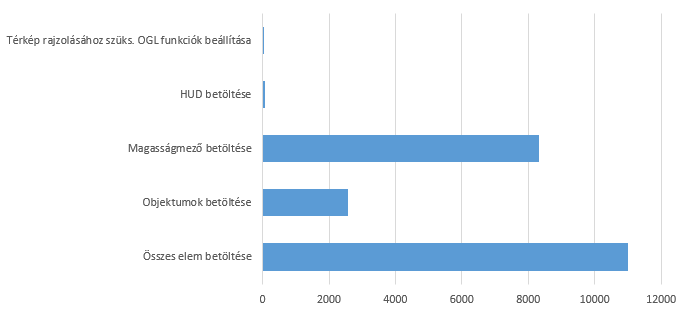
\includegraphics[scale=0.84]{kepek/map_load_diag.png}
\caption{A játéktér betöltésének ideje}
\label{fig:map_diag}
\end{figure}

Mivel a magasságmező betöltésének ideje nagyon kiugró, külön megvizsgáltam (\ref{fig:height_map_diag}-ös ábra), hogy azon belül melyik rész okozza ezt.
 
\begin{figure}[h]
\centering
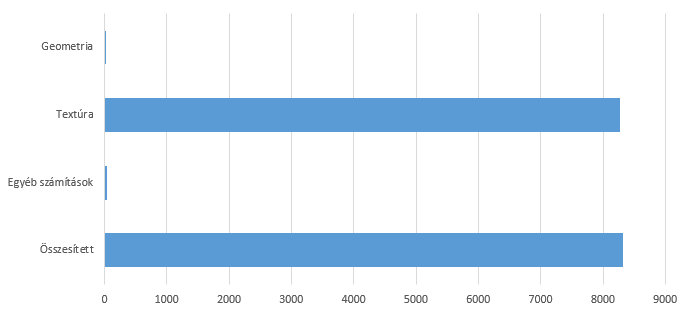
\includegraphics[scale=0.84]{kepek/height_map_load_diag.png}
\caption{A domborzat betöltésének ideje részletezve}
\label{fig:height_map_diag}
\end{figure}

Végső soron megvizsgáltam, hogy egy képkocka elkészülése során, melyik játékkomponens megjelenítése vagy számítása hogyan oszlik el a teljes képkocka idejének elkészüléséhez képest, amely fix 120 másodpercenként képkockaszám (FPS) mellett lett kiszámolva. Tudjuk, hogy 120FPS esetén a képkockák kirajzolása között eltelt időtartam 8,33ms, így elég volt csak a modellek, illetve a magasságmező kirajzolásának idejét mérni, a maradék értelem szerűen a további háttérszámításokat teszi ki.
A másik ok, ami miatt fix FPS-t választottam a méréshez, az a túl magas másodpercenkénti képkockaszám (átlag 2000FPS) korlátozás nélkül. Ilyen esetben a képkockák kirajzolása között eltelt időtartam annyira kicsi volt, hogy még milliszekundumban is mérhetetlen volt.

\begin{figure}[h]
\centering
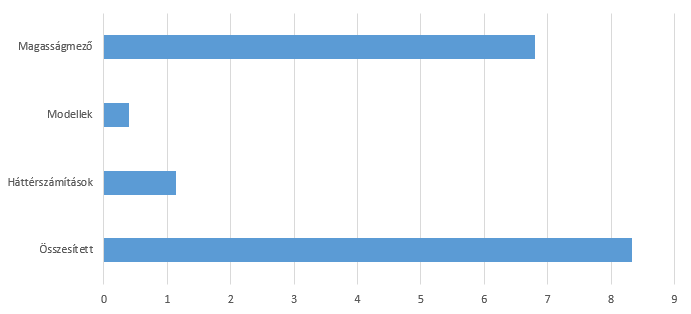
\includegraphics[scale=0.84]{kepek/frame_draw_diag.png}
\caption{Egy képkocka kirajzolása (120FPS esetén)}
\label{fig:frame_draw}
\end{figure}